\chapter[A bioinf. framework for downstream genome analysis]{A bioinformatics framework for flexible automation of downstream genome analysis}
\chaptermark{Bioinf. framework for genome analysis}
\label{chap:frameworkforgenomics}

{ \Large \leftwatermark{
\put(-67,-66.5){ 1 }
\put(-67,-91.5){ 2 }
\put(-67,-116.5){ 3 }
\put(-67,-141.5){ 4 }
\put(-67,-166.5){ 5 }
\put(-67,-191.5){ 6 }
\put(-76.5,-225){\includegraphics[scale=0.8]{img/thumbindex.eps}} \put(-67,-216.5){ {\color{white} 7 }}
\put(-67,-241.5){ 8 }
} \rightwatermark{
\put(350.5,-66.5){ 1 }
\put(350.5,-91.5){ 2 }
\put(350.5,-116.5){ 3 }
\put(350.5,-141.5){ 4 }
\put(350.5,-166.5){ 5 }
\put(350.5,-191.5){ 6 }
\put(346.5,-225){\includegraphics[scale=0.8]{img/thumbindex.eps}} \put(350.5,-216.5){ {\color{white} 7 }}
\put(350.5,-241.5){ 8 }
}}

\hfill \textsl{unpublished}

\newpage

\noindent
K. Joeri van der Velde\textsuperscript{1,2}, Lennart F. Johansson\textsuperscript{2}, Ellen Carbo\textsuperscript{3}, Bart Charbon\textsuperscript{1}, Martine Meems-Veldhuis\textsuperscript{2}, Dennis Hendriksen\textsuperscript{1}, Cleo C. van Diemen\textsuperscript{2}, Freerk van Dijk\textsuperscript{1,2}, Fleur Kelpin\textsuperscript{1}, Kristin M. Abbott\textsuperscript{2}, Birgit Sikkema-Raddatz\textsuperscript{2}, Richard J. Sinke\textsuperscript{2} and Morris A. Swertz\textsuperscript{1,2,*}\\

\noindent
1. University of Groningen, University Medical Center Groningen, Genomics Coordination Center, Groningen, The Netherlands\\
2. University of Groningen, University Medical Center Groningen, Department of Genetics, Groningen, The Netherlands\\
3. University Medical Center Utrecht, Department of Genetics, Utrecht, The Netherlands\\

\noindent
* To whom correspondence should be addressed.

\section*{Abstract}

With the popularity of next-generation sequencing rising, we expect thousands of individuals to soon have whole-genome profiling.
However,  implementation is a huge challenge for both genome research and diagnostic applications, with the primary roadblock not data acquisition or variant calling, but downstream interpretation.

Interpretation can be sped up using the huge amount of useful information collected by laboratories, public databases and biobanks. Unfortunately, for now, all these sources of useful data cannot be easily integrated and explored in unison. Further, while many innovative analysis methods emerge from research on a regular basis, a lack of standardization makes it difficult to adopt, share, compare and validate them in practice.

Here we report a lightweight framework for genome interpretation pipelines that aims to enable rapid implementation and adaptation of analysis protocols that integrate reference annotation data (e.g. ClinVar, ExAC, GoNL), run best-practice analysis tools (e.g. VAAST or GAVIN), capture their outputs in a standardized way using a new VCF extension, and use those outputs to generate informative, customizable reports for human interpretation.
Clear definitions of tools and standardization of outputs enable interoperability/flexibility and encourage members of the genomics community to jointly develop and reuse framework components in order to rapidly integrate new data and methods and develop and share new best practice protocols.
Standardized validation and benchmarking enables rapid testing and uptake of these developments.
We used MOLGENIS open source for its implementation but the framework can be readily added in other software.

Implementation of this framework in a genome diagnostic setting shows that we can successfully translate the latest knowledge and methods to medical practice.
However, we also envision its usage for different types of genomic studies because the framework is straightforward and offers advantages in terms of storing and sharing results.
Software downloads, manuals and source code can be found at \url{www.molgenis.org/genomics}.


\section{Introduction}

Sequencing of DNA and RNA has become pivotal in modern life science research, and we can now exploit our understanding of the genome to develop molecular diagnostic tests for many disorders.
However, when it comes to making more discoveries in research, there is still a need for better data integration\cite{Ritchie_2015} in order to discover new disease genes.
At the same time, in genome diagnostics, an increasing number of patients expect a reliable molecular diagnosis based on their complete genome\cite{Berg_2011} while diagnostic yield is still highly variable\cite{Wang_2014, Mart_nez_2016, Daoud_2016, Yubero_2016}.

To improve the situation, we can utilize a rapidly growing list of relevant methods, data and knowledge tools. Unfortunately, sharing and uptake of these new analysis resources is difficult because it takes considerable effort to investigate, adapt and validate them into diagnostic or research protocols.
This is partly because the quality and reusability of academic software remains low\cite{Prins_2015} while commercial software prefers to incorporate widely used methods that lag behind innovation. As a result, institutes develop their own interpretation strategies, with varying degrees of success\cite{Brownstein_2014}, to keep up with a quickly evolving field.

To encourage sharing and incorporation of community-built and commercial tools they should be easy to adopt into the interpretation workflows used in practice.
The first step to achieving this is to agree on the definitions of each processing step instead of focusing on implementations.
This has already happened for NGS variant calling pipelines\cite{Weiss_2013}, which are often composed of multiple commandline tools that are loosely connected by scripts and intermediate output files.
In NGS variant calling, steps such as aligning sequenced reads and variant calling are carried out by tools such as BWA, Samtools and GATK.
In this process, they use standard file formats FASTA/FASTQ, BAM/SAM and VCF (Variant Call Format).
This separation allows tools to be interchanged and optimized as a distinct unit of functionality in a bigger pipeline, driving innovations like Sambamba\cite{Tarasov_2015}, which is specifically developed for high-performance filtering of BAM files.

To better serve both research and routine diagnostic needs, we now wished to expand our NGS pipelines further downstream with the same modularity for fast integration and exchange of genome analysis methods such as the recently published GAVIN tool\cite{van_der_Velde_2017}.
To facilitate this, we present here a framework for standardized genomic analysis with interchangeable components.
It includes a new intermediate VCF-based format to capture relevant findings as the basis for interoperability between the tools in the pipeline, a task for which there was no pre-existing solution. We have tested and validated this framework with an open source implementation for genome diagnostics including tools for variant annotation, interpretation and reporting.


\section{Results}

\subsection{Framework for downstream genome analysis}

We developed a variant analysis framework consisting of a number of intermediate files and tool roles (annotation, analysis, and reporting).
The intermediate files use the well-known VCF specification, with additional extensions to support interoperability between alternative tools that fulfill the same role.
A new VCF extension called rVCF (Report VCF) is used to describe variants of interest.

We implemented and validated the framework into an existing bioinformatics pipeline within UMCG clinical genome diagnostics laboratory using both existing and newly developed tools.
See Figure \ref{fig:frameworkforgenomics_overview} for an overview of the components and data flow within the framework.
Below we first describe the file formats and tool roles involved and then provide examples of the implementation, usage and results of the framework as applied to genome diagnostics.\\

\begin{sidewaysfigure*}
\centering
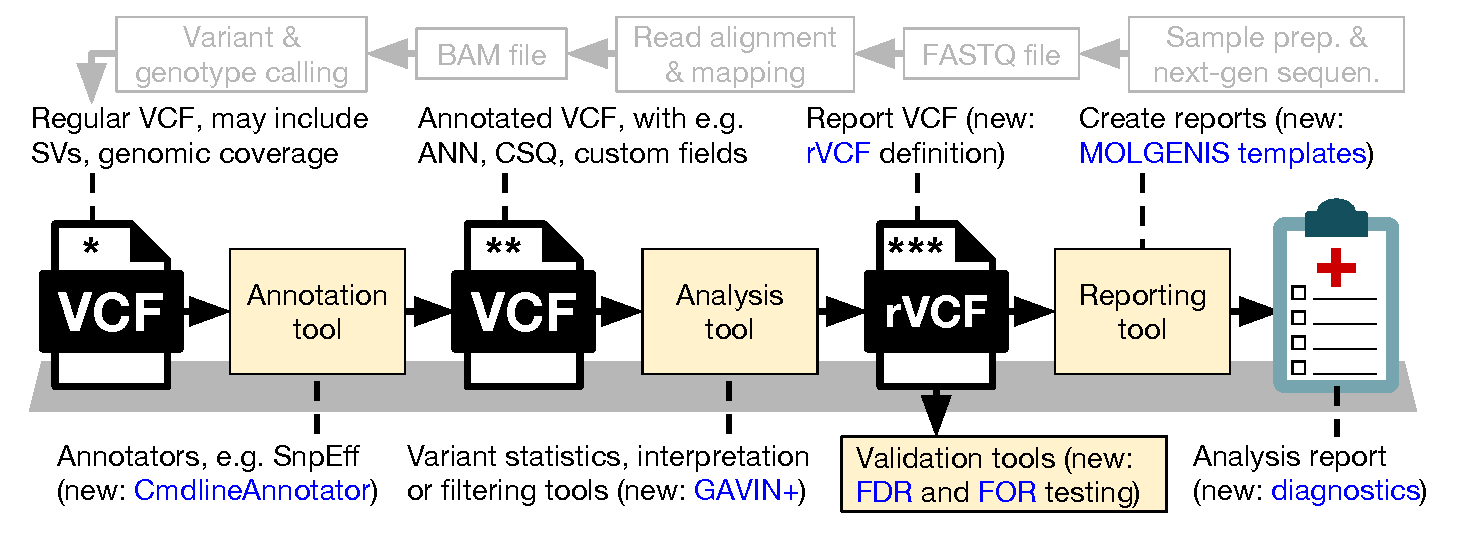
\includegraphics[width=1.0\linewidth]{img/frameworkforgenomics_overview}
\caption[Overview of the framework for automation]{Overview of the framework for adaptable automation of downstream genome analysis. New tools and formats developed for the genome diagnostic implementation of the framework are highlighted in blue. Upstream pipeline steps that are not part of the framework are shown in grey.}
\label{fig:frameworkforgenomics_overview}
\end{sidewaysfigure*}

\noindent We define the following intermediate files and tool roles: \\

\noindent\textbf{Regular VCF} files capture SNVs and small indels with the option to also capture genomic coverage and structural variants using existing definitions.
The VCF 4.2 standard\footnote{\url{https://samtools.github.io/hts-specs/VCFv4.2.pdf}} can describe any type of variation.
For genomic coverage, the gVCF\footnote{\url{https://software.broadinstitute.org/gatk/guide/article?id=4017}} extension may be used.\\

\noindent\textbf{Annotation tools} such as SnpEff\cite{Cingolani_2012}, Ensembl VEP\cite{McLaren_2010}, Jannovar\cite{J_ger_2014}, VarioWatch\cite{Cheng_2012} and CmdlineAnnotator (presented below).
These tools accept VCF files as input and add more contextual information per variant. \\

\noindent\textbf{Annotated VCF} files contain the enrichment of variants with additional contextual information from population references, known disease genes/variants, in silico pathogenicity estimates, GWAS, pathways and more.
This is stored in a standardized way to ensure tool interoperability (i.e. steps can be changed without needing to rewrite the pipeline).
We reuse existing field definitions where possible, such as the SnpEff ANN field\footnote{\url{http://snpeff.sourceforge.net/VCFannotationformat_v1.0.pdf}} and Ensembl VEP CSQ field\footnote{\url{http://www.ensembl.org/info/docs/tools/vep/vep_formats.html}}.
In addition, we added fields such as CADD\_\-SCALED (for CADD scores) and EXAC\_\-AF (for ExAC allele frequencies) for more annotations.\\

\noindent\textbf{Analysis tools} such as GE\-MI\-NI\cite{Paila_2013}, In\-ter\-Var\cite{Li_2017}, VI\-KING\cite{Miller_2015}, KGG\-Seq\cite{Li_2012}, VAAST\cite{Kennedy_2014} and GA\-VIN+ (presented below).
These tools filter and query annotated VCFs to find candidate variants.
Ideally, these tools output their results in Report VCF which can be processed or visualized further by other tools. \\

\noindent\textbf{Report VCF} files store the outcome of a genome analysis, such as GWAS p-values or diagnostic interpretation.
This intermediate file format stores relevant findings in a computer-readable format to increase pipeline flexibility by disconnecting results from reporting (see Figure \ref{fig:frameworkforgenomics_rvcfapplications}).
We build upon the VCF format by defining a specific extension for results, abbreviated 'rVCF'.
This format is fully VCF-compliant but adds an extra INFO field named RLV (relevance) that ensures tool interoperability within this framework.
This field contains the explanation for why this variant was thought to be relevant for the question imposed on the original data.

The RLV field was developed with the following criteria in mind: it should (i) be broad enough to allow many types of uses (e.g. for diagnostics, genome research, population studies); (ii) be specific enough for the results captured to be informative, at least for our diagnostic use case; (iii) provide all necessary contextual information to explain why a variant is relevant for the question posed; (iv) be structured and simple enough to allow reports to be created in a straightforward way (e.g. by templating); and (v) not contain unnecessary fields that would bloat the specification beyond its intended purpose and make it harder to use.
See Table \ref{table:frameworkforgenomics_rvcffields} for a detailed breakdown of the fields in the rVCF specification and how they can be used for different use-cases.\\

\begin{figure*}
\centering
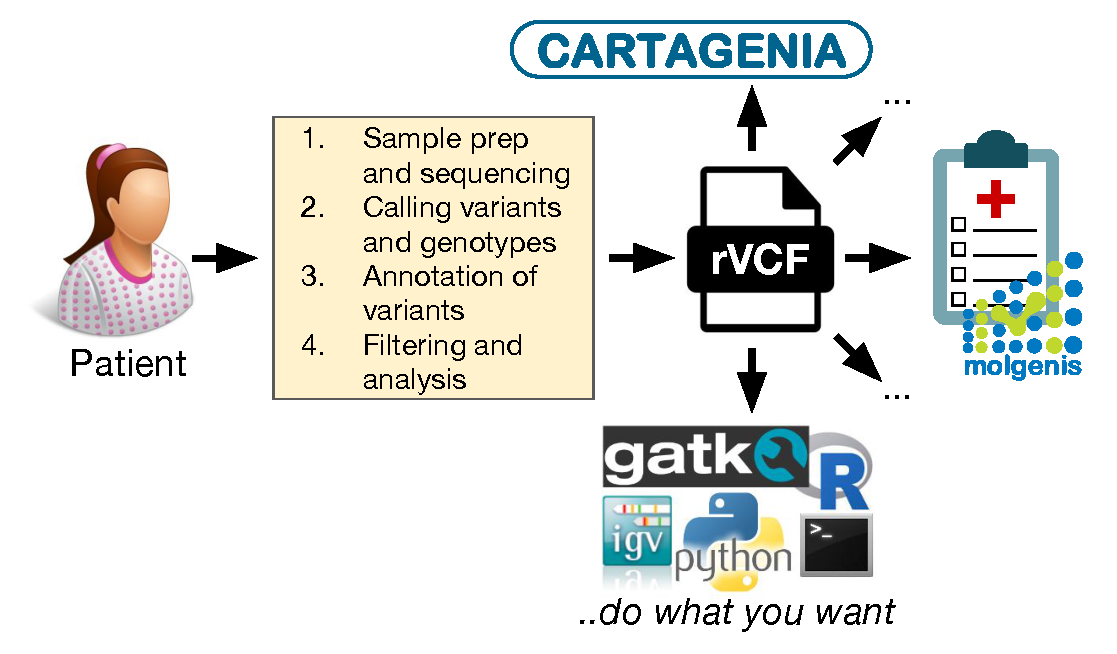
\includegraphics[width=1.0\linewidth]{img/frameworkforgenomics_rvcfapplications}
\caption[Applications of the rVCF format]{Creation and possible applications of the rVCF format. After the output has been generated by the analysis step, the results are stored in an rVCF file. This file can then be further analyzed or used to create a report. We have processed and visualized results in MOLGENIS\cite{Swertz_2010a} and Cartagenia Bench Lab\textsuperscript{TM} (Agilent Technologies), but any other tool or environment can be used including GATK\cite{Van_der_Auwera_2013}, Integrative Genomics Viewer\cite{Thorvaldsdottir_2012}, scripting languages and command line.}
\label{fig:frameworkforgenomics_rvcfapplications}
\end{figure*}

\begin{table*}
\scriptsize
\begin{tabulary}{\linewidth}{LL}
  \mbox{Field~~~~~~~~~~~~~~~~~~~~~~~~~~~~~~~~~~~~~~~~~~~~~~~~~~~~~~~~~~~~~~~~~~~~~~~~~~~~~~~~~~~~~~~~~~~} & Definition \\
  \hline
  \rule{0pt}{2.5ex}allele & The alternative allele in question, since VCF has multi-allelic sites \\
  \rule{0pt}{2.5ex}alleleFreq & Reference database minor allele frequencies, e.g. ExAC, GoNL or 1000G \\
  \rule{0pt}{2.5ex}gene & Gene name or identifier, e.g. HGNC symbol or MIM accession \\
  \rule{0pt}{2.5ex}FDR & Any pre-calculated FDR thresholds for this variant, gene or transcript \\
  \rule{0pt}{2.5ex}transcript & Transcript used, e.g. SnpEff canonical transcript \\
  \rule{0pt}{2.5ex}phenotype & Trait of disorder in question, e.g. trichotillomania, BMI or ethosuximide resistant \\
  \rule{0pt}{2.5ex}phenotypeInheritance & Mode of inheritance, e.g. dominant, recessive, additive \\
  \rule{0pt}{2.5ex}phenotypeOnset & Age of onset, e.g. pediatric, adult, L2-stage \\
  \rule{0pt}{2.5ex}phenotypeDetails & Extra phenotype info, e.g. treatment options or literature references \\
  \rule{0pt}{2.5ex}phenotypeGroup & Grouping of phenotypes, e.g. cardiovascular, neurological, oncological \\
  \rule{0pt}{2.5ex}$<many>$ sampleStatus & How this sample is potentially affected based on genotype and inheritance e.g. HOMZYG, AFFECTED, COMPOUND, DENOVO, CARRIER \\
  \rule{0pt}{2.5ex}$<many>$ samplePhenotype & The actual sample phenotype, taken from VCF 'SAMPLE' annotation field \\
  \rule{0pt}{2.5ex}$<many>$ sampleGenotype & Sample variant or marker genotypes with possibly quality or probability data \\
  \rule{0pt}{2.5ex}$<many>$ sampleGroup & Grouping of samples, e.g. case, control, EUR, AFR, infant, adult \\
  \rule{0pt}{2.5ex}variantSignificance & Type or value of variant significance, e.g. Reported pathogenic, Predicted pathogenic, pval 0.0035 \\
  \rule{0pt}{2.5ex}variantSignificanceSource & Tool or source used to discover this variant, e.g. your lab list, ClinVar, PolyPhen2, CADD, SIFT, GAVIN \\
  \rule{0pt}{2.5ex}variantSignificanceJustification & The reason why source thought this variant was interesting, or the criteria used by prediction tool \\
  \rule{0pt}{2.5ex}variantMultiGenic & Denote how this variant is potentially part of digenic or other complex forms of inheritance \\
  \rule{0pt}{2.5ex}variantGroup & Grouping of variants, e.g. suggestive, significant, iarc\_\-class\_\-5 \\
  \hline
\end{tabulary}
\caption[rVCF format specification]{rVCF format. Interoperability is ensured by standardizing interpretation information within the framework using a new 'RLV' field. Within this field, specific interpretation data can be described using the VCF standard INFO sub-field structure. Any sub-fields marked with $<many>$ may contain multiple values, each linked to specific sample identifiers. Multiple RLV values may be present to accommodate multi-allelic variants and overlapping gene annotations.}
\label{table:frameworkforgenomics_rvcffields}
\end{table*}

\noindent\textbf{Reporting tools} turn Report VCF into result overviews that can be read by human users and tailored to a specific audience.
A database system such as MOLGENIS, for example, can import, store, query and share genomic data and analysis results, then format it for diagnostics reporting from a diagnostics lab in a way that the clinical geneticist can use.
The system can be used to create analysis reports from the stored results.\\

\noindent\textbf{Analysis reports} are the final products of the downstream analysis.
They can be clinical patient reports for doctors or statistical genome-wide reports for researchers.
Multiple reports for different users and questions may be generated from an analysis, and within a report there is no limit on flexibility or interactivity, although use of single file documents with a simple and well-thought out graphical layout is encouraged.\\

\noindent\textbf{Validation tools} (automatically) test and evaluate pipeline results in a standardized way against a gold-standard data set.
Such validation is a precondition for diagnostics implementation.
Examples of possible validation tests include a false omission test to count how many expected hits were actually observed in the Report VCF output, a false discovery test to see how many unexpected hits were found, or a combination of the two.
These tests can be executed on individual level, on gene level, or across the whole genomes of many individuals simultaneously.
Validations of the pipeline are (automatically) performed whenever software versions or data sources have been updated.

\subsection{Implementation for genome diagnostics}

We used this framework to implement an automated downstream analysis and reporting pipeline for genome diagnostics.
Below we describe examples of annotation, analysis and reporting tools that are connected by using the standardized interpretation data format.

\subsubsection{Annotation tool: CmdlineAnnotator}

We implemented a high-performance tool that performs annotation tasks that enable variant enrichment.
It wraps common genomic annotation sources, such as ExAC\cite{Lek_2016}, 1000 Ge\-nomes\cite{Auton_2015}, Ge\-nome of the Ne\-ther\-lands\cite{Francioli_2014}, Clin\-Var\cite{Landrum_2015} and CADD\cite{Kircher_2014} in a standardized way. 
This enables us to quickly add and combine different annotation steps, which was one of our goals with this framework.
The tool, MOLGENIS CmdlineAnnotator, can be run on command line making it easy to script into typical bioinformatic pipelines, but we have also implemented a web interface for interactive use.
The tool requires no installation other than downloading an executable, and its use is straightforward.
MOLGENIS CmdlineAnnotator supports any valid VCF file, handles multi-allelic variants and can match equivalent variants even when their notation is different (see Methods and Materials).

\subsubsection{Analysis tool: GAVIN+}

We also created a new analysis tool to replace the analysis protocol we had used before.
GAVIN+ is a diagnostic interpretation tool that prioritizes DNA variants of potential clinical relevance in the genome.
It achieves this by using GAVIN\cite{van_der_Velde_2017}, a sensitive tool to predict pathogenic variants based on gene-specific CADD scores calibrated on ExAC, ClinVar and SnpEff.
In addition, GAVIN+ matches against candidates against known pathogenic variants in ClinVar but removes potential false positives with a GoNL/ExAC $>$5\% MAF.
The tool then queries the Clinical Genomics Database\cite{Solomon_2013} to find affected and carrier individuals depending on sample genotype and mode of inheritance.
For uncharacterized genes, the default heterozygous, compound heterozygous and homozygous states are assigned.
Depending on the input VCF, additional knowledge is automatically used.
This includes trio-aware sample filtering and genotype phasing to check validity of compound heterozygous hits, or reassigning status from, e.g., ‘homozygous by compound mutation’ back to ‘multiple hits on the same allele’.
Hemizygous genotypes for chromosome X and Y are also taken into consideration.
The tool even works on mitochondrial genotypes, albeit with limited references.
We run GAVIN+ as a command line runnable standalone tool that takes an annotated VCF file and returns a Report VCF file.

\subsubsection{Report VCF: novel format}

The Report VCF (rVCF) format is used to mark variants that may be of clinical interest.
The field that captures the clinical relevance, which is similar to SnpEff's ANN field, consists of a single string with multiple sub-fields separated by pipe symbols.
The values are described in the VCF header and include the alternative allele in question, gene, and transcript (just as in ANN), but rVCF also includes associated phenotype, inheritance mode, onset, genotype and affected/carrier status of samples, reason why this variant was relevant and according to whom.

There are currently 19 values within the RLV field, but in practice the notation is quite compact because unused sub-fields add only one character to the notation.
See Table \ref{table:frameworkforgenomics_rvcfdata} for examples of comparable VCF INFO field extensions for the same variant, including an example of the RLV field.

\begin{table*}
\begin{tabulary}{\linewidth}{LL}
  VCF INFO field & Data example \\
  \hline
  Consequence annotations from Ensembl VEP & CSQ=T $|$ 5\_\-prime\_\-UTR\_\-variant $|$ MODIFIER $|$ UROS $|$ ENSG00000188690 $|$ Transcript $|$ ENST00000368797 $|$ protein\_\-coding $|$ 1/10 $| | | |$ 7 $| | | | | | |$ -1 $| |$ HGNC $|$ 12592; \\
  ~ & ~ \\
  Functional annotations from SnpEff & ANN=T $|$ 5\_\-prime\_\-UTR\_\-variant $|$ MODIFIER $|$ UROS $|$ UROS $|$ transcript $|$ NM\_\-000375.2 $|$ Coding $|$ 1/10 $|$ c.-219C$>$A $| | | | |$ 6722 $|$; \\
  ~ & ~ \\
  Relevance annotations from GAVIN+ & RLV=T $|$ 0.0 $|$ UROS $|$ 0.0 0.011980830670926517 $|$ NM\_\-000375.2 $|$ Porphyria congenital erythropoietic $|$ RECESSIVE $|$ Pediatric $| | |$ DNA7654321:CARRIER $| |$ DNA7654321:0s1 $| |$ Reported pathogenic $|$ ClinVar $|$ NM\_\-000375.2(UROS):c.-219C$>$A UROS Pathogenic $| |$; \\
  \hline
\end{tabulary}
\caption[Examples of VCF INFO field definitions]{Examples of VCF INFO field definitions. The VEP consequence and SnpEff annotation fields describe the functional effects of a variant on genes and transcripts at its locus. The relevance field denotes why this particular variant and effect was included in the analysis result, such as screening for candidates that may explain a clinical phenotype.}
\label{table:frameworkforgenomics_rvcfdata}
\end{table*}

Because all applicable sample genotypes in question are now stored in the RLV field,  information on the genotype used is left out of the rVCF file.
The data reduction achieved by selecting only variants of potential relevance is substantial, and turns out very relevant for usage in a health care setting.
For example, on a data set of samples from 69 patients that were sequenced for panel of 96 dystonia genes, we reduce 2,154 variants (6.3 megabyte, MB) to 63 variants (90 kilobyte, kB).
A patient exome of 108,004 variants (77 MB) was reduced to 449 variants (625 kB), and a combined VCF with 282 exomes of 790,297 variants (7.3 GB) was reduced to 19,572 variants (17 MB).
In research one might still want to retain all data, therefore we developed a helper tool to merge the rVCF files back into the full list of variants and genotypes in the original VCF file, which provides more flexibility for how the format can be used.
Another helper tool can split the compound RLV field into many separate info fields for ease of import and filtering in other tools.

\subsubsection{Reporting tool: patient report for genome diagnostics}

We have implemented a report generator to visualize the information contained within rVCF using the MOLGENIS web database, although interested readers can easily write their own.
The rVCF files can be uploaded and stored in the database just like any other VCF file.
After importing, the genomic data can be browsed, queried, visualized and filtered using standard MOLGENIS UI components in the Data Explorer.
In addition, users can generate reports based on a simple template language (FreeMarker) and use R, Python or JavaScript and web services to make very interactive reports.
These templates can be uploaded, customized, changed, and reused within the database itself.

We have defined a patient report template that transforms the data into an overview showing the main findings of potential clinical relevance.
This report ranks the variants by importance for medical interpretation based on the evidence from the data and how well genes and variants are clinically characterized\cite{McLaughlin_2014}.
Users can apply a number of post-filters within the report if needed.
For instance, they may wish to exclude or include certain genes, e.g. those for late-onset disorders in the case of a young patient, or adjust the variant MAF inclusion threshold.
See Figure \ref{fig:frameworkforgenomics_patientreport} for an example of this report.

\begin{sidewaysfigure*}
\centering
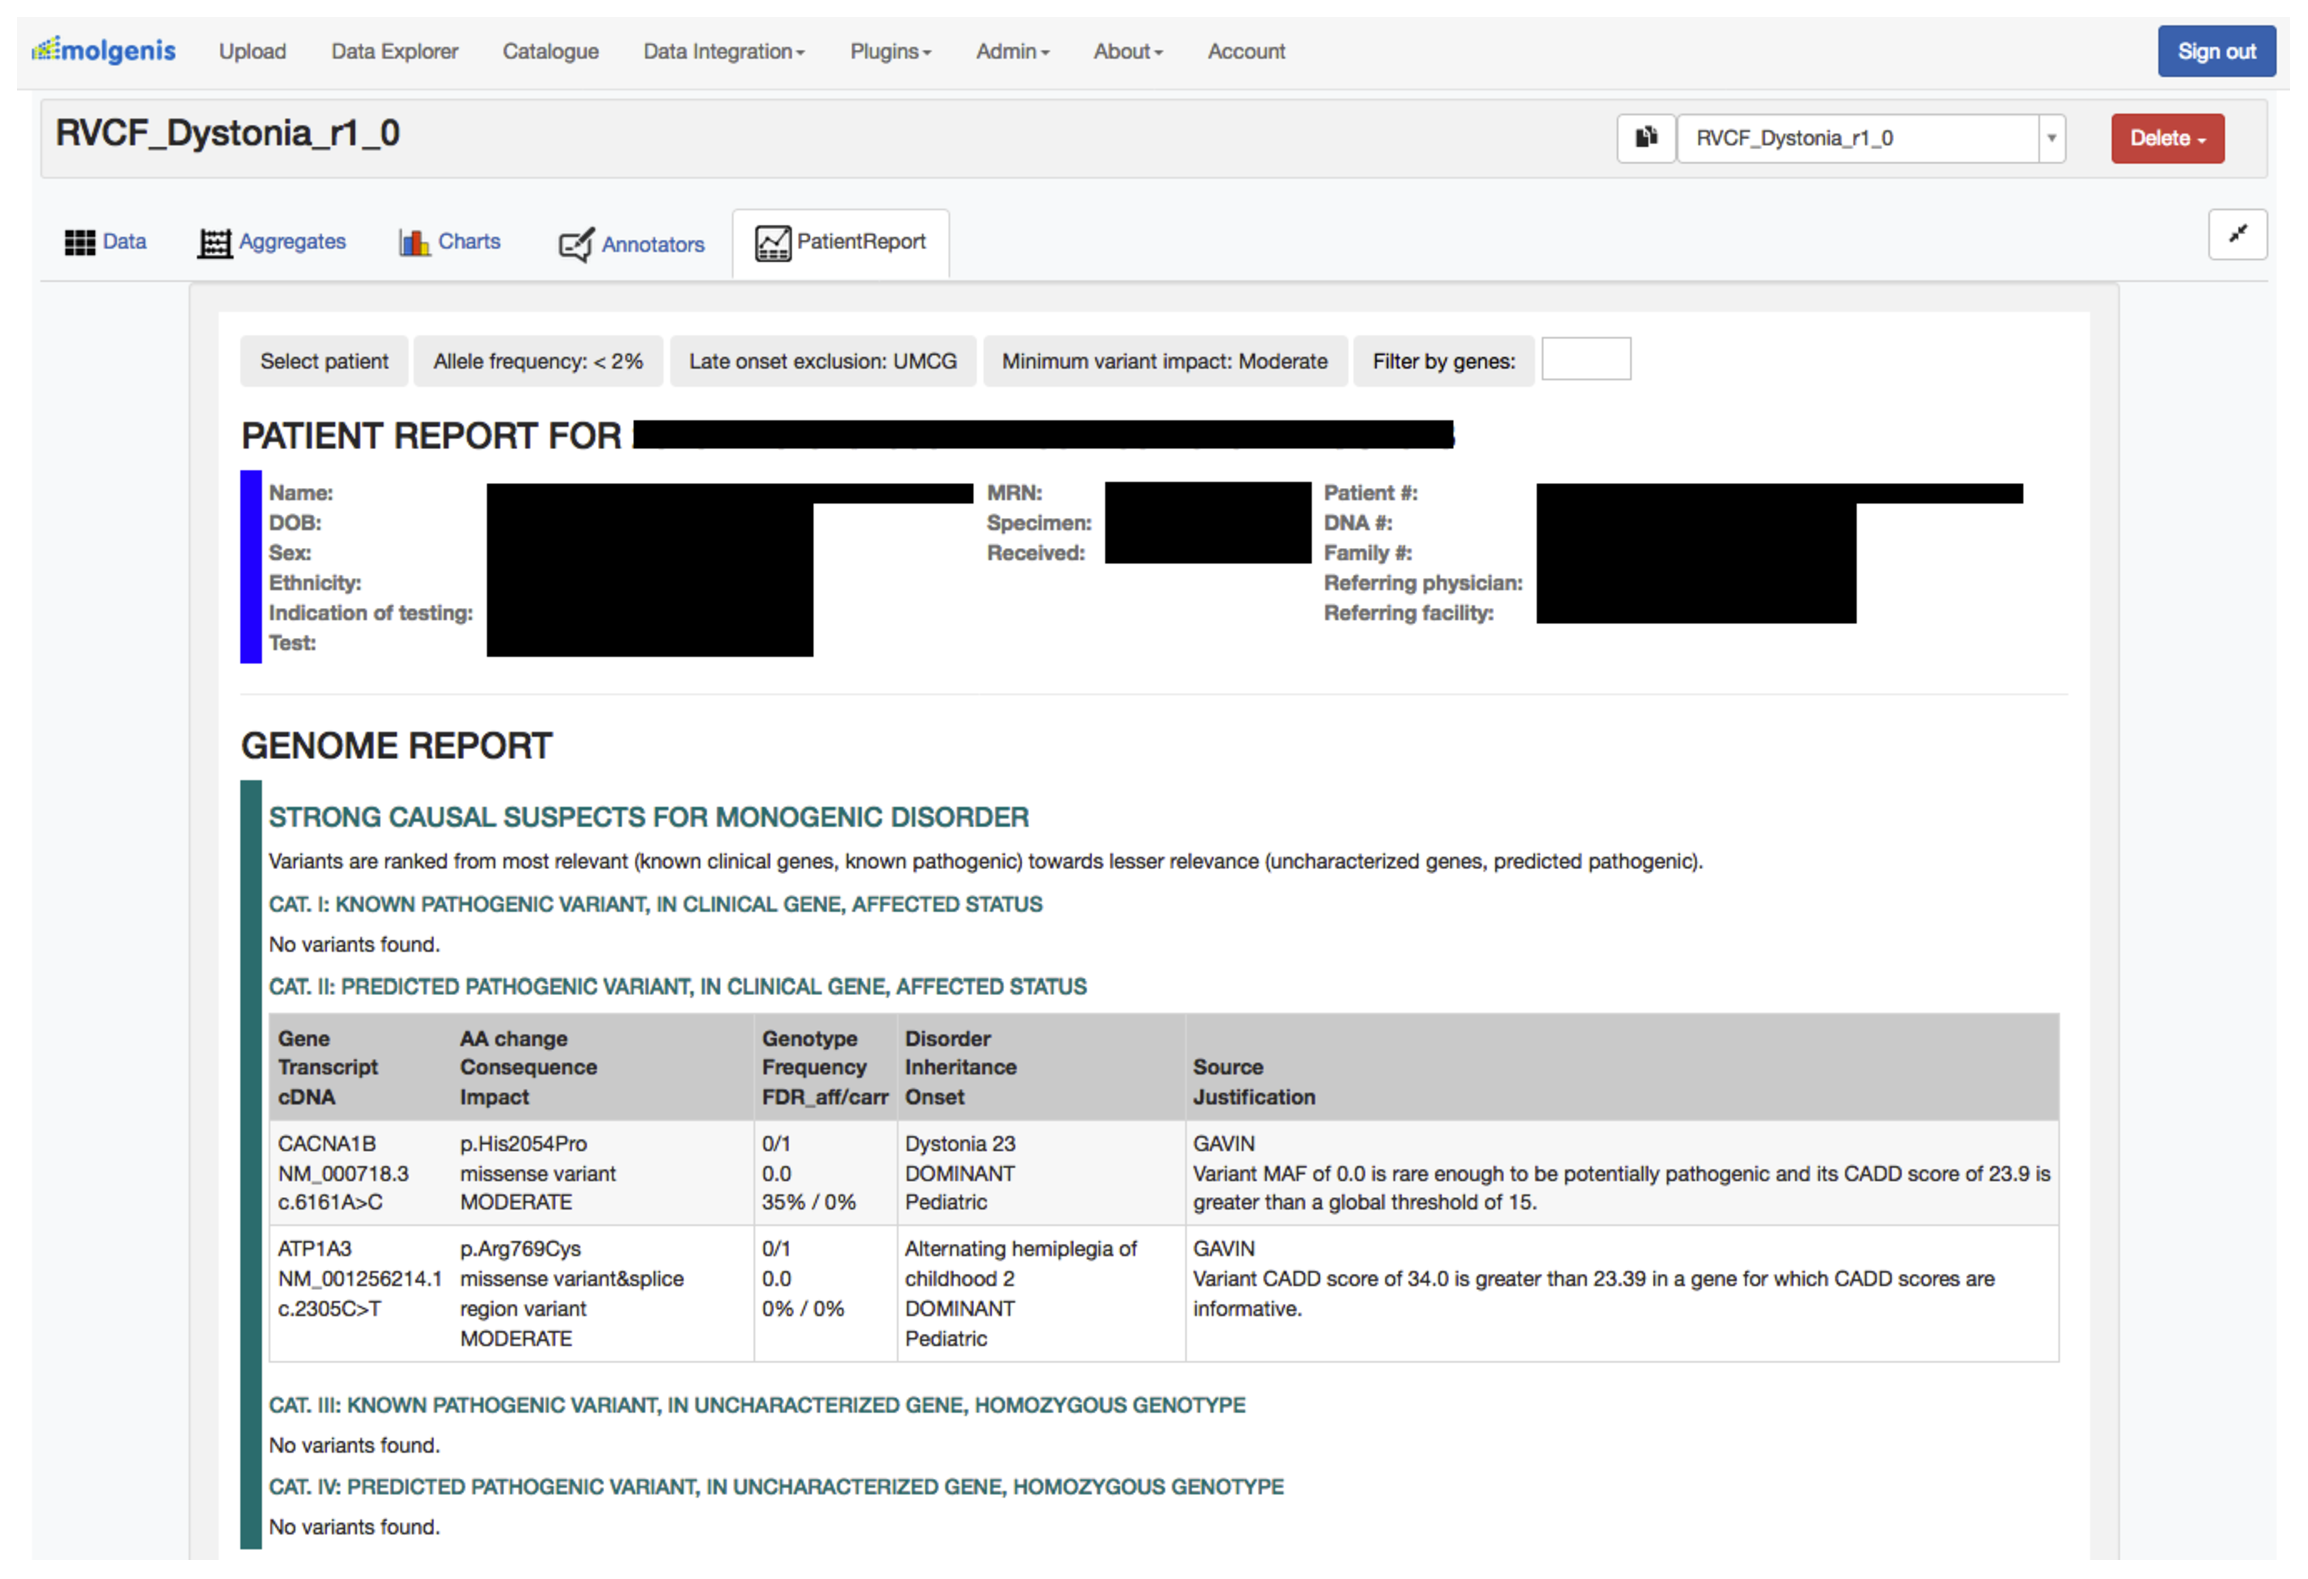
\includegraphics[width=1.0\linewidth]{img/frameworkforgenomics_patientreport}
\caption[Example screenshot of a patient report]{Example screenshot of a patient report generated in MOLGENIS. Sensitive information has been blacked out. Reports are created fully automatically using a template engine on an imported rVCF data set. The buttons at the top offers post-render customization options.}
\label{fig:frameworkforgenomics_patientreport}
\end{sidewaysfigure*}

\subsection{Validation tool: evaluation for diagnostics}

Establishing a molecular diagnosis is only possible when enough data is filtered out to allow human interpretation of the remainder while maintaining reasonably confidence that computational pre-filtering did not remove the causal variant.
To estimate the number of variants that were not detected (false negatives or missed), and the number of variants incorrectly implicated (false positives) in our pipeline implementation for genome diagnostics, we set up an automated validation procedure.
These validations can be quickly run as many times as needed to check performance and expected output of pipelines whenever they undergo any change or update.
This allows efficient testing and uptake of new methods for clinical use, which should increase diagnostic yield.

\subsubsection{Estimation of false omission}

First we investigate how many of the pathogenic variants that we want to find are actually detected.
A missed detection, or false omission, is the most worrisome type of error for molecular geneticists and other experts because a diagnosis cannot be established.\\

\noindent\textbf{Public benchmark data}\\
We performed a false omission rate (FOR) analysis on the GAVIN+ interpretation tool (version 1.0) using known pathogenic variants.
First, we calculated gene-specific FOR on the GAVIN\cite{van_der_Velde_2017} benchmark set, a comprehensive gold-standard consisting of 8,087 unique pathogenic variants from various sources (VariBench, ClinVar, MutationTaster and UMCG clinic), in 1,113 genes.
In total we detected 7,598 of the 8,087 (94\%) pathogenic variants. For 889 (out of 1,113) genes we recovered all their variants, meaning these genes have a FOR of 0\%.\\

\noindent\textbf{In-house patient variant list}\\
As an additional analysis, we exported the most recent controlled in-house list of interpreted variants from our current clinical diagnostic interpretation software.
In this list there were 980 unique variants classified as Pathogenic or Likely pathogenic.
We recall 936 of these 980 variants, or 95.5\%, consistent with the previous result.
See Figure \ref{fig:frameworkforgenomics_for} for an overview of false omission counts per gene.\\

\begin{sidewaysfigure*}
\centering
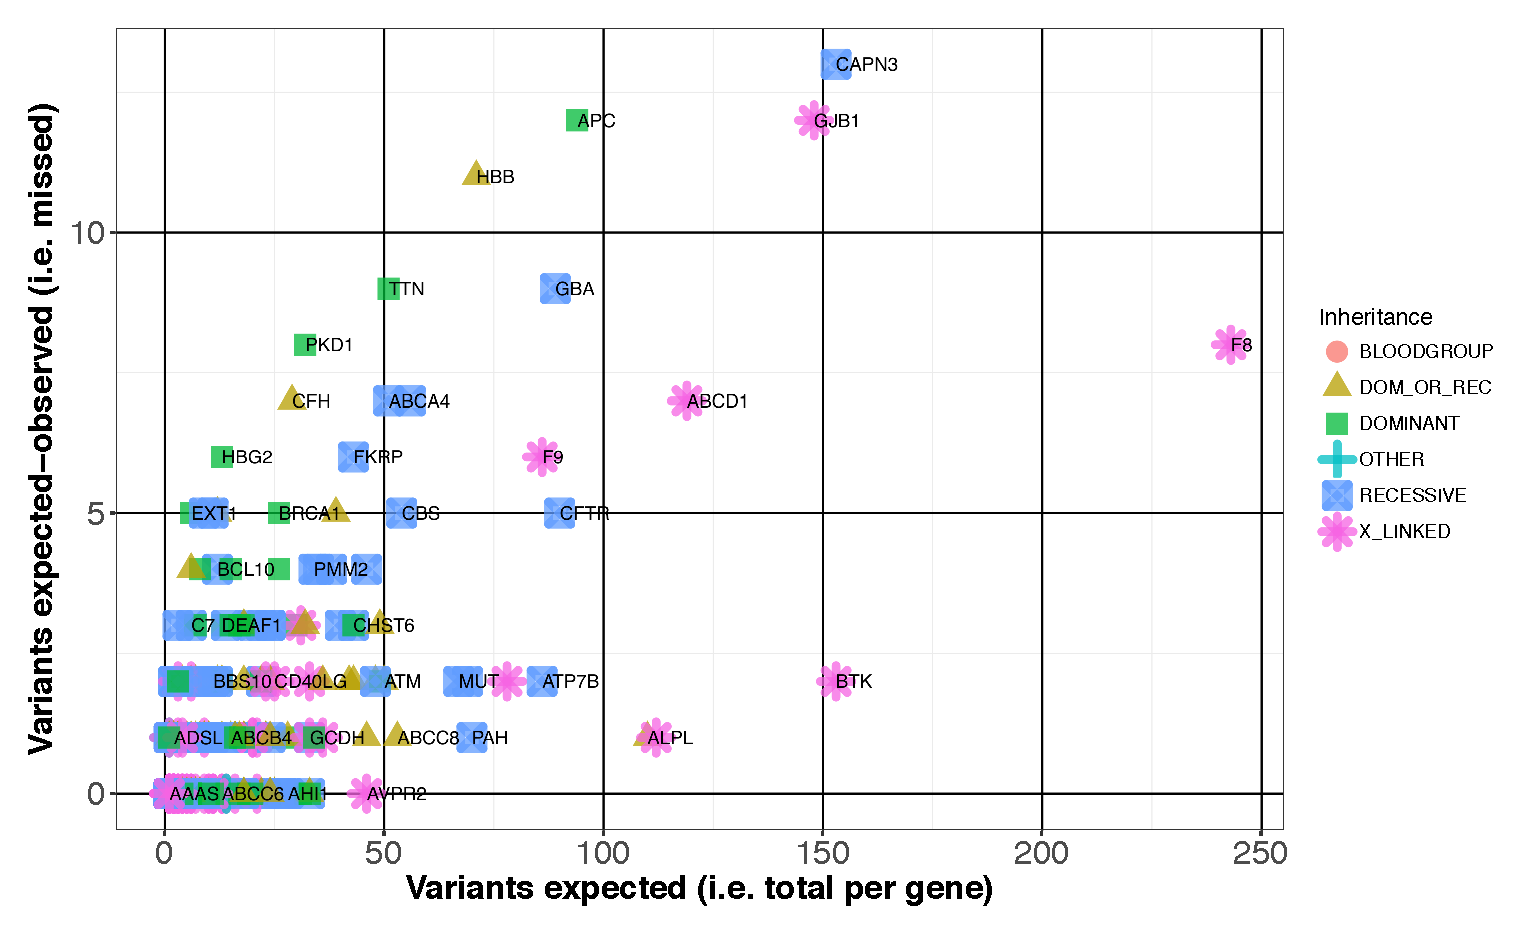
\includegraphics[width=1.0\linewidth]{img/frameworkforgenomics_for}
\caption[GAVIN+ false omission on pathogenic variants]{Counts of GAVIN+ false omission on known pathogenic benchmark variants. Shown are 1,048 (out of 1,113) genes with known inheritance modes from the Clinical Genomics Database.}
\label{fig:frameworkforgenomics_for}
\end{sidewaysfigure*}

\noindent\textbf{In-house patient cases}\\
Lastly, we gathered diagnostic results of 31 patients for whom whole genome or whole exome sequencing was performed to find the molecular cause of their diseases.
These include 21 adults from our clinic (2x pulmonary arterial hypertension, 2x familial cancer, 1x familial hypercholesterolemia, 2x epilepsy, 2x dystonia, 2x epidermolysis bullosa, 10x cardiomyopathy) and 10 critically ill newborns and infants from our rapid genome sequencing program\cite{van_Diemen_2017}.
Executing our diagnostic implementation of the framework resulted in a small number of hits that was checked by molecular geneticists.
In the adult patients, we retrieved the causal pathogenic variant in 18 of 21 cases.
For the 10 newborns, we found the correct mutation in all 10 cases.
In total, we recalled 28 out of 31 variants, or 90\%.
The variants that were missed can be found in Table \ref{table:frameworkforgenomics_missedpatientvariants}.

\begin{sidewaystable}
\begin{tabulary}{\linewidth}{LLLLLL}
  \mbox{Gene~~~~~~~~~} & \mbox{Variant~~~~~~~~~~~} & \mbox{Expert opinion~~~~~~~~~~~~~~~~~~~~~~~~~} & Reason missed & Gene FOR benchmark \\
  \hline
  \rule{0pt}{2.5ex}TTN & c.68225-1G$>$C (splice acceptor-site variant) & Likely pathogenic & Variant CADD score of 24.3 is less than 26.93 in a gene for which CADD scores are informative & 51 / 43 / 15.7\% \\
  \rule{0pt}{2.5ex}NPC1 & c.3011C$>$T (protein change p.Ser1004Leu) & Pathogenic & Variant MAF of 9.39E-4 is greater than 4.36E-4 & 3 / 3 / 0.0\% \\
  \rule{0pt}{2.5ex}LDLR & c.-135C$>$G (5' UTR promoter variant) & Pathogenic & Variant CADD score of 12.88 is less than 16.13 in a gene for which CADD scores are informative & 43 / 41 / 4.7\% \\
  \hline
\end{tabulary}
\caption[Variants that were missed by the GAVIN+]{Variants that were missed by the GAVIN+ interpretation tool. In two instances, CADD scores were in the benign range and in one case the MAF was just too high to be considered pathogenic. The gene FOR benchmark column shows the false omission test results for the corresponding gene as number of variants expected, number recalled and percentage missed (E / R / M\%).}
\label{table:frameworkforgenomics_missedpatientvariants}
\end{sidewaystable}

\subsubsection{Estimation of false discovery}

To gain confidence in our method to predict a variant to be pathogenic for a patient, we estimated how often it would return false hits in genomes of healthy individuals.
A hit here means a potentially pathogenic variant under an acting genotype, e.g. heterozygous for a dominant disorder or homozygous for a recessive disorder.
A very low or even zero number of positive hits in healthy individuals would increase the chance that a hit found in a patient is indeed causal for disease.\\

\noindent\textbf{Public reference genomes}\\
To estimate the gene-specific false discovery rate (FDR) of the interpretation pipeline, we used 2,504 healthy individuals who were whole-genome sequenced in the 1000 Genomes Project\cite{Auton_2015}.
In total, we used 38,097,906 non-intergenic variants observed across chromosomes 1-22, X, Y, and MT.
Per gene, we counted how many unique samples would have one or more variants detected as potentially pathogenic.
This may happen in affected status, meaning that the genotype matches the known inheritance mode of a clinical gene, or if the sample has a homozygous genotype.
For carrier status, the sample is heterozygous, which cannot occur for dominant acting genes.
When applied to the GAVIN+ interpretation tool (version 1.0) described above, we find a mean affected fraction of 0.26\% with a median of 0\%, and a mean carrier fraction is 1.85\% with a median of 0.72\%.
For an overview of gene-specific false discovery rates, see Figure \ref{fig:frameworkforgenomics_fdr}.\\

\begin{sidewaysfigure*}
\centering
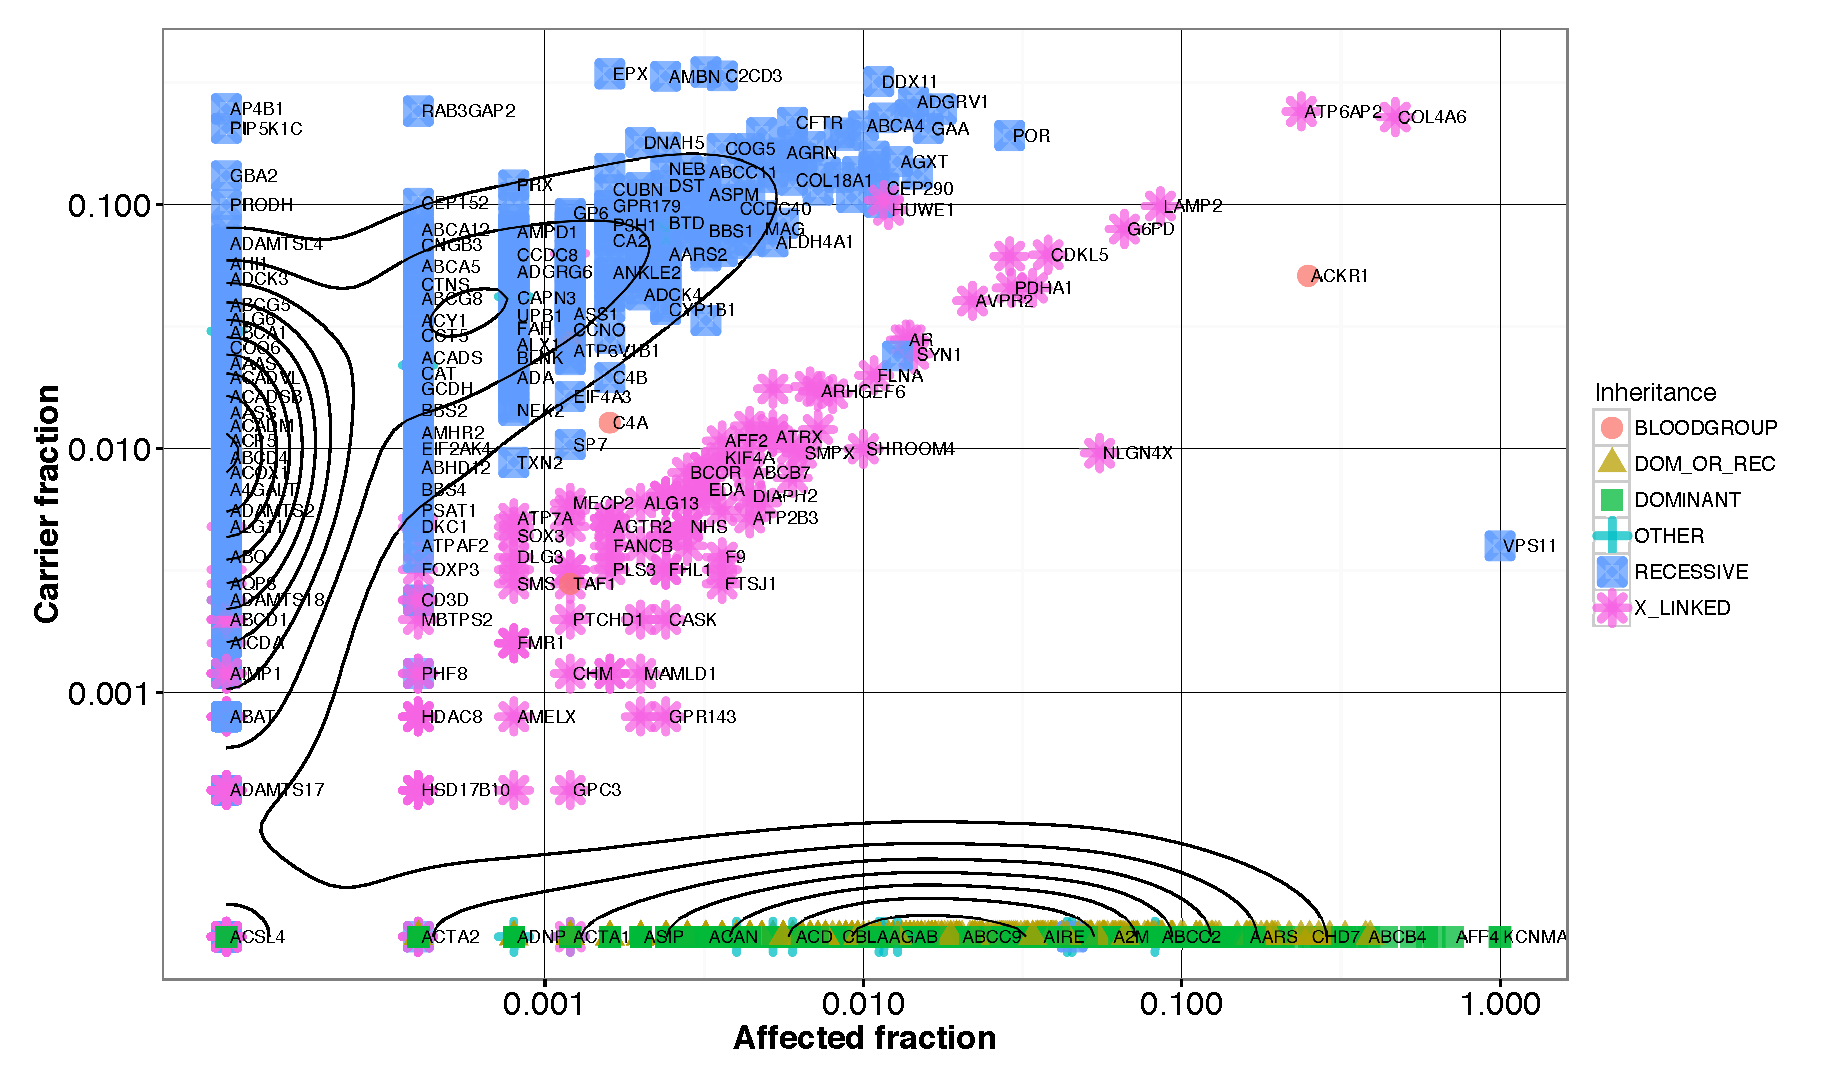
\includegraphics[width=1.0\linewidth]{img/frameworkforgenomics_fdr}
\caption[Estimations of GAVIN+ false discovery rate]{Estimations of GAVIN+ false discovery rate using data from the 1000 Genomes Project. Each point represents the fraction of affected vs. carrier samples, i.e. the number of samples for which a potentially pathogenic genotype was detected under that inheritance mode within a specific gene, divided by the total number of samples. Only genes with known inheritance modes in the Clinical Genomics Database are shown.}
\label{fig:frameworkforgenomics_fdr}
\end{sidewaysfigure*}

\noindent\textbf{In-house patient variant list}\\
We also performed an additional assessment on an in-house list of variants classified by experts (for details, see Methods and Materials).
These variants were rare enough for careful assessment by clinical geneticists as candidates for potential disease-causing effects but were found to be plausibly harmless.
Of the 9,145 variants classified as benign or likely benign, the tool reports 336 hits, resulting in a false positive rate of 3.7\%.


\section{Discussion}

We have reported our development a conceptual framework for structured, automated interpretation of variants with interchangeable components loosely connected by the VCF format.
In addition, we created a first implementation of the framework building on the existing open source MOLGENIS software.
We integrated existing commandline tools as well as a number of new software tools for annotation, analysis and filtering into an executable pipeline for genome diagnostics.
The newly proposed rVCF extension provides an interoperability backbone and, importantly, adds the previously missing link by including information that explains why variants were part of the analysis results.
Furthermore, all rVCF files can be loaded into a web database that generates a report for researchers that provides an overview of clinically relevant findings for medical use.
The content of the reports can be adjusted using option menus, or fully customized by programmers using a template system.
By default, the reports rank variants from most relevant to least relevant.

We have proven our approach with a functional result, but both the framework and its implementation have sparked many ideas for further improvement.
Below we discuss the framework itself, evaluate the implementation results and finally provide direction for future work.

\subsection{Framework considerations}

\subsubsection{Tool interoperability}
The framework defines how tools and data fulfill specific roles within the context of genome interpretation.
However, it does not specify if and how the output of one tool can be connected to the expected inputs of another.
While some output fields are standardized to a degree, such as SnpEff’s 'ANN' field, others are custom or even ambiguous.
For example, an 'AF' field probably refers to allele frequency, but does not make explicit from which population reference this frequency is taken.
An internationally recognized and maintained list of annotation fields might solve this ambiguity, but this agreement needs support from the entire community and requires software changes in most existing tools.
A subtler but easier to achieve strategy would be to use an ontology of genomic annotations to which user can map their software output fields.
To use a familiar reference point, Sequence Ontology\cite{Eilbeck_2005} could be extended with genomic annotations, organized in categories such as 'computational predictions' and 'population allele frequencies'.
In this way, different output annotations could point towards a common reference and software implementations could migrate over time without breaking backwards compatibility.

\subsubsection{Report VCF format}
rVCF specification was defined to capture the relation of any phenotype to any variant including the context in which this association was established.
The information included in rVCF was based on clinically relevant information such as disease phenotype and inheritance, affected individuals, their genotypes, and the reason why this variant was selected.
The data captured in this format can be used to generate genomic reports.
We believe the specification can be easily adopted by other genomic use-cases such as genome-wide association studies (GWAS), quantitative trait loci (QTL) studies, linkage studies or epigenetic studies.
Examples of values for domains other than genome diagnostics, such as model organisms or statistical associations, are shown in Table \ref{table:frameworkforgenomics_rvcffields}.
While the format should be able to accommodate all these applications, additional fields may need to be incorporated to capture important information.
We are curious to find out what these extra requirements are, and we cordially invite the community to adopt, standardize, provide feedback about and improve upon the format.

\subsection{Implementation enhancements}

\subsubsection{Detailed validation output}
The validation tools presented produce false positives and false negatives percentages either overall or per gene.
However, this does not provide insight into the exact differences between the old and a new pipeline or the types of errors made.
To gain more insight, such tools should create a report of their own that compares the errors of the previous pipeline version with the current version.
Information such as 'there is a 14\% increase in false negative splice variants but a 20\% decrease in false positive missense variants' can be very helpful for further improvements or a second tier test to mitigate a particular flaw.

\subsubsection{False discovery analysis}

The GAVIN+ tool was also applied to 2,504 healthy genomes to estimate the rate of false discovery, i.e. to give an indication of how many falsely accused variants can be expected for each gene (see Figure \ref{fig:frameworkforgenomics_fdr}). 
However, since the 1000 Genomes data is based on low-coverage sequencing, it is unclear whether the false positives we found are caused by flaws in our method or by false genotypes present in the data.
Thus, the resulting plot might reflect sequencing bias or genotype calling errors instead of the actual limitations of our method.
To make these estimates more comparable and representative of the data used in a diagnostic sequencing, we need high-coverage whole-genome data from many thousands of  healthy individuals from all ethnic backgrounds.
With the current data, causal variants might be dismissed because of undeservedly high false discovery estimates of the genes they are in.
Another approach that could be used is to use population genomes as a background from which we may calculate diagnostic significance \textsl{P} values for individual patient genomes\cite{Wilfert_2016}.

\subsubsection{Phenotype-matched reports}
The framework implementation we have presented uses only genomic information to generate a patient or research report.
Of course, the clinical features of the sample offer vital clues as to which gene is likely responsible for the disease.
It would therefore make sense to include phenotype-based gene filtering or prioritization to the report.
To make this possible, associations of Human Phenotype Ontology (HPO) terms\cite{Robinson_2010} to their known disease genes could be integrated into the system.
Users can enter HPO terms that match the phenotypes observed in a patient to shorten their list of candidate genes.

\subsection{Increasing diagnostic yield}

\subsubsection{Reducing false positives}
False positives in the context of genome diagnostics are harmless variants that are mistaken for pathogenic.
Predicting many variants as pathogenic translates to a high workload for human experts, who must manually investigate variants before communicating the results to the patient.
To decrease the number of false positives, we can also use specific populations like those provided within ExAC and 1000 Genomes instead of population-wide allele frequency thresholds.
Variants that may be relatively common in one sub-population but not present in others could be filtered out, having low overall MAFs but would logically be considered harmless.
However, with fewer individuals used to ascertain the frequency of a variant within a specific population, the potential bias introduced by randomly including non-representative samples also increases.
This can be addressed by calculating confidence intervals for allele frequencies, and using those in practice instead of the direct allele frequency values.

In addition,  population reference databases such as ExAC offer not only allele counts but also counts of observed homozygous and heterozygous genotypes.
For recessive disease genes, the number of observed homozygous genotypes may be more informative than allele frequency, as the variant may be carried within the population without pathogenic effect.

Lastly, another improvement that could reduce the number of false positives is checking for variants or sequencing artifacts previously classified as benign in ClinVar or other sources such as in-house variant lists.

\subsubsection{Reducing false negatives}
False negatives in the context of genome diagnostics are pathogenic variants that are not detected, a type of error that must be strongly avoided.
The number of false negatives could be reduced by built-in consideration of pathogenic founder mutations.
These can be common enough for a MAF cutoff filter to accidentally remove them before interpretation.
Reporting these variants in international or local databases for use as an interpretation safety net, which is already an optional input for the GAVIN+ interpretation tool, would resolve this issue to a degree.
UMCG genome diagnostics uses an in-house list to identify such variants, but an internationally shared and curated list would be an improvement.

While it is unfortunate that some variants can be missed, estimating miss rates does provide an \textsl{a priori} measure of the difficulty of finding pathogenic variants in their respective genes.
Variants in genes with high estimated miss rates can be double checked when patient symptoms point toward these genes as likely candidates.
This knowledge turns \textsl{unknown unknowns} into \textsl{known unknowns}, empowering the interpretation process and shedding light on potential uncertainties.

\subsubsection{Using structural variation}
This study was focused on processing single-nucleotide variants (SNVs) and small indels, but the structural variation (SV) output of tools such as Manta\cite{Chen_2015} and Delly\cite{Rausch_2012} would also be an important addition to automated interpretation framework.
The regions indicated to be deletions, insertions, duplications, inversions or translocations may be complemented with any SNVs and small indels called by conventional variant callers to increase overall diagnostic yield or to obtain a more complete genomic picture for research projects.

\section{Conclusion}

We have developed and evaluated a framework for structured, stepwise downstream variant analysis.
The aim was a structure that links the different tools and data in this process to enable exchange, reuse and improvement of components of equal scope across institutes.
The novel rVCF intermediate format allows standardized representation of analysis results, and these can be used to quickly create patient or research reports.
We expect that this modular structure will also make it easier to integrate the additional omics technologies that will soon support next-generation sequencing, such as allele specific expression and splicing effects from RNA-sequencing expression, epigenetic markers and metabolomics.

Geneticists have already adopted and learned to rely on best-practice pipelines for NGS variant- and genotype-calling, partly because these tools have matured by the efforts and support of the community but primarily because there is too much raw data to assess by hand.
Given the ever-growing numbers of whole-genome patient sequences we must extend this mentality further downstream towards analysis and interpretation.
To deal with false positives and negatives more effectively, our approach includes automated validation and error estimation tools applied to large benchmark sets to assess the quality and pitfalls of such a pipeline.
We have shown that our diagnostic framework implementation combines and automates the latest knowledge, tools and practices to reduce the time and effort spent on easily resolvable patient cases, a  times savings that will provide human experts with the time they need to solve puzzling cases that will further extend our knowledge of human genetics.


\section{Methods and Materials}

\subsection{MOLGENIS annotation tool}
We developed MOLGENIS CmdlineAnnotator as an extensible annotation framework that works seamlessly in both web and commandline environments.
It has some smart features to maximize the match of input variants (patient) to resource data (context) such as population references.
As an example we can consider the case where the annotation resource has a variant $AGG>A,ATGG$ to denote both the deletion of $GG$ and the insertion of $T$ and our input VCF file has a $A>AT$ variant at the same location.
Though this variant is present in the resource, it would likely be missed because the notation is different.
The CmdlineAnnotator matches this variant by removing but remembering $GG$ from $AGG$ to match the input $A$.
The input alternative allele $AT$ would subsequently be postfixed with $GG$ to form $ATGG$, which matches against the resource successfully.
These slight but relevant differences can be responsible for misinterpretation during analysis.
CmdlineAnnotator version 1.21.1 source code and release are available at \url{https://github.com/molgenis/molgenis/releases/tag/v1.21.1}.

\subsection{Population reference for false discovery analysis}
We downloaded the 1000 Genomes Project phase 3\cite{Auton_2015} release data from \url{ftp://ftp.1000genomes.ebi.ac.uk/vol1/ftp/release/20130502/}.
We annotated genes using SnpEff version 4.2 with these settings: hg19 -noStats -noLog -lof -canon -no-intergenic -ud 0.
Allele frequencies of Genome of the Netherlands\cite{Francioli_2014} release 5 and ExAC\cite{Lek_2016} release 0.3, and CADD scores\cite{Kircher_2014} version 1.3 were annotated using MOLGENIS CmdlineAnnotator v1.21.1.
All VCF FORMAT fields except genotype (GT) were removed from chromosome X and Y to harmonize the data with chromosomes 1-22.
Also, the genotyped samples for chromosomes Y and MT are different from those in chromosomes 1-22.
We wrote a simple tool (SampleFixFor1000GchrYandMT.java) to harmonize the samples for Y and MT, available at \url{https://github.com/molgenis/gavin-plus}.
These fixes now allow all data to be merged by stripping the headers and concatenating the files in the order 1-22, X, Y and MT.
The header from chromosome 1 was added to the merged file with a few INFO lines added that were specific for other chromosomes: LEN, TYPE and OLD\_\-VARIANT from chromosome X, and VT from chromosome MT.
The resulting file was compressed to 8.4G with bgzip and indexed using tabix -p vcf.
It contains 38,097,906 non-intergenic variants and 95,397,156,624 genotypes.
The file is available at \url{http://molgenis.org/downloads/gavin/}.

\subsection{Pathogenic variants for false omission analysis}
We used the GAVIN\cite{van_der_Velde_2017} variant classification benchmark set available at \url{https://github.com/molgenis/gavin}.
This set comprises 25,995 variants from which we select 8,087 pathogenic variants after filtering duplicate genomic positions.
We annotated these variants with SnpEff 4.2, ExAC r0.3, CADD 1.3 and GoNL r5 using MOLGENIS 1.21.1 CmdlineAnnotator.
A heterozygous genotype was added to each variant to enable running of the GAVIN+ automated interpretation tool.
This dataset is available for download at \url{http://molgenis.org/downloads/gavin/}.

We also used a list of variants interpreted by molecular and clinical geneticists at the University Medical Center Groningen according to Dutch medical center guidelines\cite{ACGN}.
More details on the interpretation criteria are provided in Van der Velde \textsl{et al.}\cite{van_der_Velde_2017}.
This list contained 980 likely pathogenic or pathogenic variants and 9,145 benign or likely benign variants after filtering for duplicate genomic positions.
These variants were annotated and processed as above, and access to these data can be requested.

\subsection{GAVIN+ interpretation tool}
We developed the GAVIN+ tool to automate sample genome interpretation.
In a stepwise process, interesting variants are selected (based on hits from GAVIN\cite{van_der_Velde_2017}, ClinVar\cite{Landrum_2015}, or a user-supplied list of variants), followed by a MAF filter, match of genotype to gene inheritance mode, checks for compound heterozygosity and the use of trio or duo sample genotype phasing and de novo variant finding.
GAVIN+ supports multiple alleles per variant that may be present in multiple overlapping gene annotations.
It is implemented in Java 1.8 (\url{https://www.java.com}) as free open source software at \url{https://github.com/molgenis/gavin-plus}.
A comprehensive TestNG (\url{http://testng.org}) test suite ensures correctness and allows further development with a limited chance of introducing bugs.
Dependencies are managed by Apache Maven (\url{https://maven.apache.org/}).
A precompiled, command line runnable version of the tool can be downloaded at \url{http://molgenis.org/downloads/gavin/}.
A demo and manual are available, as are the bundled resources needed to run the tool: ClinVar (any variant matching 'pathogenic' from combined TSV and VCF representations of 11 oct. 2016, 1.5 MB), CGD (version 11 oct. 2016, 380 kB), FDR (version 1.0, 946 kB) and GAVIN calibrations (r0.3, 331 kB).
The implementation insures high performance by using a streaming architecture with as little in-memory buffering as necessary and as much output as possible immediately written to disk.
This results in speeds of millions of genotypes per second.
 GAVIN+ can analyze 300 whole exomes in ~2 minutes or the full 1000G FDR analysis (95,397,156,624 genotypes) in ~2 hours on commodity hardware.

\subsection{Running false omission analysis}
We ran the GAVIN+ tool in a first pass (using -m CREATEFILEFORCADD) to get a list of 34 indel variants that are not yet scored by CADD.
These variants were then scored by a local CADD 1.3 which was installed offline following the instructions at \url{http://cadd.gs.washington.edu/download}.
After scoring, GAVIN+ was run for a second and final pass using arguments: -i GAVIN\_\-FOR\_\-benchmark\_\-goldstandard\_\-nodup\_\-gonl.vcf -g bundle\_\-r1.0/GAVIN\_\-calibrations\_\-r0.3.tsv -c bundle\_\-r1.0/clinvar.patho.fix.11oct2016.vcf.gz -d bundle\_\-r1.0/CGD\_\-11\-oct\-2016\-.txt\-.gz -a fromCadd.tsv -f bundle\_\-r1.0/FDR\_\-allGenes\_\-r1.0.tsv -m ANALYSIS -o RVCF\_\-GAVIN\_\-FOR\_\-benchmark\_\-goldstandard\_\-nodup\_\-gonl\_\-r1.0\-.vcf.
This was followed by a simple tool (FOR.java, available at \url{https://github.com/molgenis/gavin-plus}) to report the false omission rate using original VCF and the rVCF file produced by the GAVIN+ tool.
For each gene, we counted the number of pathogenic variants in the original VCF that we expect to recover.
We divide this number by the observed number of variants in the rVCF as a missed fraction for each gene to estimate how well GAVIN+ detection works for that gene.
All files and results are available at \url{http://molgenis.org/downloads/gavin/}.

\subsection{Running false discovery analysis}
We ran the GAVIN+ tool in a first pass on the 1000G population reference set and got 1,136,050 variants that were not yet scored by CADD.
The local CADD 1.3 tool scored 1,110,509 (97.75\%) of these, meaning that 25,541 of 38,097,906 total variants (0.067\%) remained un-scored.
This allowed GAVIN+ to be run in a second and final pass (using -m ANALYSIS) of the data, resulting in an rVCF file with 381,482 selected variants.
To obtain false discovery rate estimates, we wrote FDR.java, a simple tool that assumes that the hits in the rVCF file are false.
These hits are counted per gene as the number of samples that would have at least one matching genotype under one of two inheritance modes.
A sample is counted as affected when the match is homozygous or compound heterozygous or heterozygous in a known dominant disease causing gene, and counted as carrier when heterozygous in either a recessive disease causing gene or an unknown gene.
A check on phasing may revert compound heterozygotes back to carrier heterozygous multihit status.
The FDR tool outputs a list of 19,230 genes, each with four columns: affected count, carrier count, affected fraction (aff.count/2504) and carrier fraction (carr.count/2504).
Among these 19,230 genes, we find 8,399 with one or more affected samples, 17,878 with one or more carriers, and an overlap of 7,047 genes (17878+(8399-7047)=19230).
This list is further processed to include all 26,023 SnpEff gene names present in the original VCF for which no affected or carrier status was detected.
This was done by first extracting all gene names using GetAllGeneNamesFromVCF.java, followed by using CombineFDRwithAllGenes.java to get the final FDR result file with 26,044 genes.
Note that 21 mitochondrial genes were present in the rVCF file due to ClinVar hits, but these were not annotated by SnpEff in the original VCF file, hence the final result includes slightly more genes.
All result files and intermediates are available at \url{http://molgenis.org/downloads/gavin/}.

\subsection{Visualizing FOR and FDR analysis results}
We wrote a small R script (FDR\_\-plot.R) that uses the FDR result file with 26,044 genes as well as gene annotations from Clinical Genomics Database\cite{Solomon_2013} (file date: August 31, 2016) to plot the observed affected versus carrier fractions.
After merging with CGD we could plot 3,232 of these genes with known inheritance modes.
The color and shape of the points is dependent on the inheritance mode, scales are base 10 logarithmic.
Zero values were replaced with 1e-4 to allow logarithmic scale.
Some genes appear in unexpected plot locations, but can be logically explained.
For instance, CSF2RA appears in the recessive band while being on chromosome X but it is located in the X-PAR1 region.
Conversely, TENM1 appears in the X\_\-LINKED band with a blue icon because it has a mistakenly RECESSIVE annotation.
For only the plotted CGD genes, we find a mean affected fraction of 1.51\% with a median of 0.08\% and a mean carrier fraction of 1.43\% with a median of 0.20\%.
Another R script (FOR\_\-plot.R) visualizes the FOR result file with 1,113 genes.
After merging with CGD we can plot 1,048 of these genes with known inheritance modes.
Again the color and shape of the points is dependent on the inheritance mode.
All scripts and required files are available at \url{https://github.com/molgenis/gavin-plus}.

\subsection{MOLGENIS reporting tool}
To store and visualize the rVCF files produced, we used a modified version of MOLGENIS 1.21.2\cite{Swertz_2010a}.
Users can simply import rVCF files via the standard Data Importer, which can then be viewed in the Data Explorer.
To create the custom reports, we used the Free\-Marker template engine (\url{http://freemarker.org}).
The templates should be placed in the mol\-gen\-is/mol\-gen\-is-app/\-src/\-main/\-resources/\-templates/ folder, and adhere to this naming scheme: view\-[report\-name]\-entities\-report.ftl.
For instance, a Patient\-Report should be named view\-Patient\-Report\-entities\-report.ftl.
The templates are then added as an additional tab for a dataset by clicking the Configure button, and in the Reports box define this link using [report\-name]:[data\-set\-name].
For instance, we connect the Patient\-Report to an rVCF named Cardio using Cardio:\-Patient\-Report.
Multiple links can be separated using commas, e.g. My\-Research\-Exomes:\-Gene\-Report,\-Dystonia:Patient\-Report,\-Cardio:\-Patient\-Report.
The used MOLGENIS and created templates are available at \url{http://github.com/joerivandervelde/molgenis}.

\section*{Acknowledgements}
We thank Kate McIntyre for editing.

\section*{Funding}
We thank BBMRI-NL for sponsoring the above software development via a voucher.
BBMRI-NL is a research infrastructure financed by the Netherlands Organization for Scientific Research (NWO), grant number 184.033.111.
We also thank NWO VIDI grant number 016.156.455.
We acknowledge the support from the Netherlands CardioVascular Research Initiative: "the Dutch Heart Foundation, Dutch Federation of University Medical Centres, the Netherlands Organisation for Health Research and Development and the Royal Netherlands Academy of Sciences" for the GENIUS project "Generating the best evidence-based pharmaceutical targets for atherosclerosis" (CVON2011-19).

\subsection*{Authors' contributions}
KJV, MS designed the conceptual framework.
KJV, BC, DH and FK developed the software and processed the data.
MMV, CCvD, KMA and BSR performed patient DNA variant interpretation and diagnostic validation.
KJV drafted the manuscript with input from LFJ, EC, DH, FvD, FK, KMA, BSR, RJS and MAS.
All authors contributed to the development of the framework and evaluated one or more components.
All authors read and approved the final manuscript.

\section*{Competing interests}
The authors declare that they have no competing interests.
